\chapter{Fundamentação Teórica}



\section{Linguagem de programação}
Uma linguagem de programação é uma linguagem artificial usada para controlar o comportamento de uma máquina. Aquele que manipula a máquina por meio de linguagens de programação é chamado de programador. Na prática, programadores utilizam linguagens de programação a fim de solucionar problemas de um determinado domínio. Há uma vasta gama de linguagens disponíveis a serem utilizadas, portanto os programadores devem possuir a capacidade de analisar e entender o problema tratado a fim de se escolher a linguagem mais adequada à situação \cite{Sebesta2011}. 

As linguagens costumam ser separadas em relação ao seu grau de abstração, quanto maior for a abstração, mais o programa escrito será intuitivo e se assemelha-rá com a linguagem falada; entretanto, maiores também serão os detalhes que se tornam inacessíveis ao programador. São chamadas linguagens de alto nível aquelas que possuem algo grau de abstração, enquanto que linguagens de baixo nível são aquelas que possuem pouca ou nenhuma abstração.
Os códigos criados devem passar por um processo de tradução antes de serem executados, com a finalidade de serem entendidos pelo computador. Para isso, são utilizados (Figura \ref{fig:compilador_interpretador}):
\begin{itemize}
    \item \textbf{compiladores}, método no qual o código fonte é traduzido em linguagem de máquina, a qual pode ser executada diretamente no computador \cite{Sebesta2011}. Um compilador traduz código escrito em uma linguagem de programação para uma forma mais adequada para execução na máquina \cite{Sipser2012-gl}.
    \item \textbf{interpretadores}, método em que o código fonte é avaliado diretamente em tempo de execução ao invés de ocorrer um processo de tradução \cite{Jones2020-iq}.
\end{itemize}

\begin{figure}
    \centering
    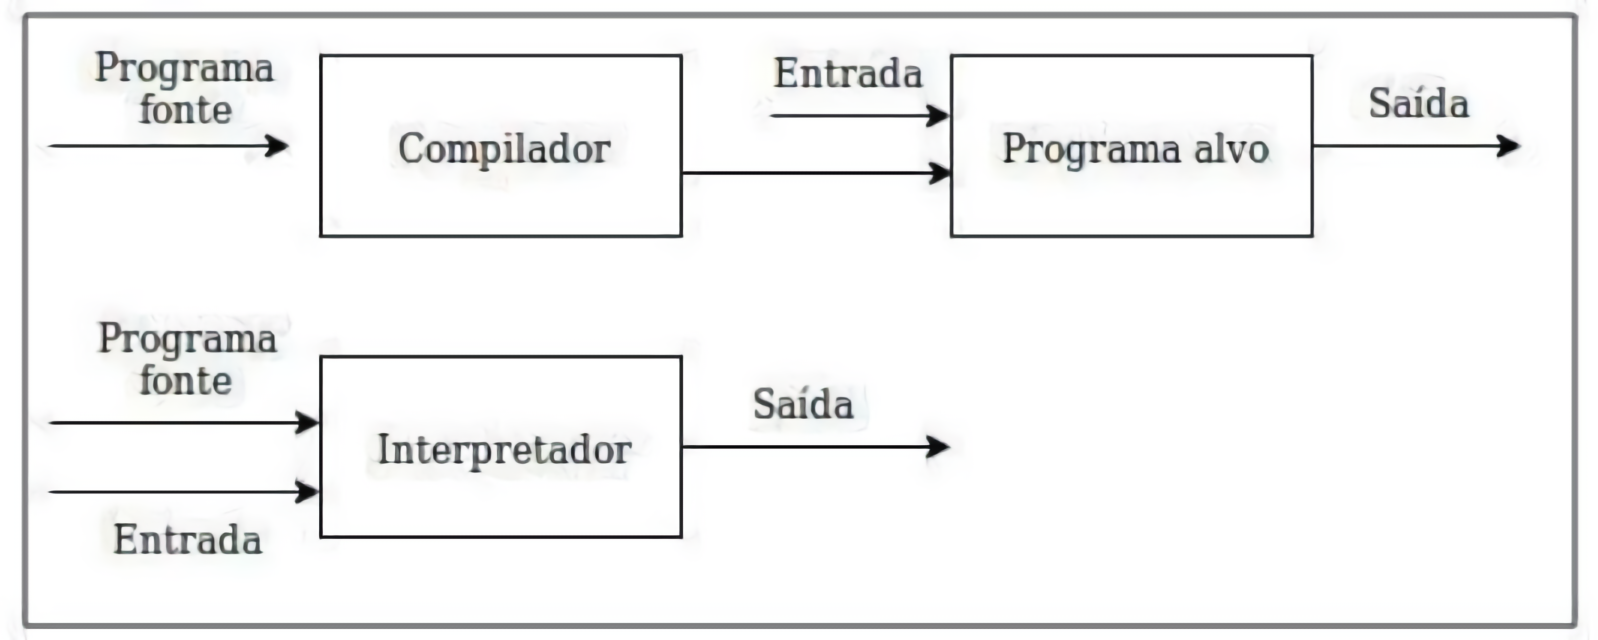
\includegraphics[width=1\textwidth]{img/Cap2/compilador_interpretador.png}
    \caption{Diferença entre compiladores e interpretadores \cite{Miotto2019}}
    \label{fig:compilador_interpretador}
\end{figure}


\subsection{Python}
Python é uma linguagem de programação de propósito geral 
e multiparadigma lançada originalmente em 1991 por Guido van Rossum, estando atualmente em sua terceira versão. Sendo uma linguagem de alto nível, sua filosofia está ligada ao fato de tornar o código mais legível e expressivo, objetivo que é atingido por via de sua sintaxe, muito se assemelhando à linguagem falada. Possui diversas estruturas de alto nível de maneira nativa, como listas, dicionários, data/hora, complexos, dentre outros \cite{Borges2010}, além de ser extensível com o uso de bibliotecas e \emph{frameworks} de terceiros. 

Possui código aberto, significando que Python pode ser livremente usado e modificado por qualquer pessoa. Com isso, a comunidade em volta da linguagem é bem expressiva e engajada. Bibliotecas e \emph{frameworks} possuem forte suporte e costumam ser bem documentados.

\subsection{Solidity}
Solidity é uma linguagem de alto nível orientada a contrato. Ela é utilizada para a implementação de contratos inteligentes (\emph{smart contracts}), sendo atualmente a principal linguagem da plataforma Ethereum \cite{Dannen2017-eb}. É realizada uma compilação a partir dos códigos gerados nessa linguagem a fim de se implantar um contrato inteligente em uma rede Blockchain.

Criada por Gavin Wood, é uma linguagem explicitamente feita para a escrita de contratos inteligentes com funcionalidades a dar suporte direto à execução em ambientes descentralizados Ethereum \cite{Antonopoulos2018-jt}.

\section{Bibliotecas e \emph{frameworks}}

Uma biblioteca é uma coleção de recursos (arquivos, classes, funções) disponível a ser utilizada em um ambiente de programação de computadores. Para \cite{Sommerville2011}, bibliotecas são consideradas como uma questão de implementação no projeto de desenvolvimento de um software. Uma destas questões é o reúso de código fonte já existente. Por se tratar de uma coleção de recursos, programadores podem optar por utilizar bibliotecas prontas ao invés de necessitar implementar as funcionalidades necessárias de um determinado domínio, poupando assim tempo e esforço.

\emph{Frameworks}, por sua vez, são coleções de classes abstratas e concretas que são adaptadas e estendidas para criar sistemas de aplicação \cite{Sommerville2011}. Costumam possuir uma ou mais bibliotecas, além de serem a estrutura mínima necessária para a implementação de projetos diversos. Podem ser vistos como uma espécie de "miniarquitetura" reutilizável que serve como base para e a partir da qual outros padrões de projeto podem ser aplicados \cite{Pressman2021-jj}. \emph{Frameworks} possibilitam a integração, por meio de código, de outros elementos, para a implementação de funcionalidades específicas.

\subsection{Flask}
Flask é um \emph{framework} destinado à web escrito na linguagem de programação Python. Costuma ser chamado de \emph{microframework} pois não necessita de bibliotecas ou ferramentas específicas por padrão. Isto dá uma grande liberdade ao programador, que possui autonomia de implementar suas soluções sem se prender a padrões intrínsecos reforçados por outros \emph{frameworks}.

O \emph{framework} foi projetado desde o seu início para ser extensível, fornecendo um núcleo robusto que inclui funcionalidades básicas necessárias por todas as aplicações baseadas no ecossistema web \cite{Grinberg2018-nz}. Não possui nativamente suporte para acessar bancos de dados, validar formulários, autenticação de usuários, dentre outras tarefas de alto nível \cite{Grinberg2018-nz}. Para isso, são utilizadas extensões fornecidas pela comunidade, que se integram transparentemente com o núcleo do \emph{framework}.

\section{Docker}
O Docker é um mecanismo de conteinerização de código aberto, que automatiza o empacotamento, envio e implantação de quaisquer aplicativos de software \cite{Raj2015-ju}. Em termos práticos, Docker é uma ferramenta que emprega virtualização a nível de sistema operacional, isolando aplicações em estruturas chamadas de contêineres; isto garante que as aplicações sejam executadas de forma isolada, agregando as dependências necessárias dentro do próprio contêiner (como expresso na Figura \ref{fig:docker_diagrama}), evitando assim problemas provenientes de conflitos de versões de bibliotecas.

O Docker foi construído em cima do kernel do sistema operacional Linux, garantindo assim acesso às suas principais funcionalidades, o que promove uma alta eficiência em seu gerenciamento de contêineres. O uso de \emph{namespaces} e \emph{cgroups} dá ao Docker uma alta capacidade de isolar recursos globais do sistema uns dos outros \cite{Raj2015-ju}. Um contêiner Docker é formado a partir de uma imagem Docker. Uma imagem é uma coleção de todos os arquivos que juntos formam uma aplicação de \emph{software}.

\begin{figure}
    \centering
    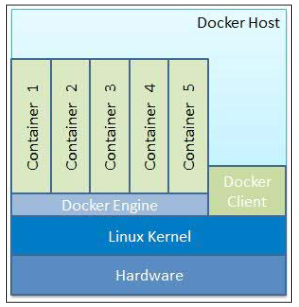
\includegraphics[width=0.45\textwidth]{img/Cap2/Docker Diagrama.png}
    \caption{Demonstração do funcionamento do Docker \cite{Raj2015-ju}}
    \label{fig:docker_diagrama}
\end{figure}

\section{API REST}
REST, acrônimo para \emph{Representational State Transfer} é o nome de um estilo arquitetural para a web elaborado por Roy Fielding em sua dissertação de Ph.D. \cite{Masse2011-cf}. Nela, Fielding detalhou seis características necessárias para sua arquitetura \cite{Grinberg2018-nz}:

\begin{itemize}
    \item \textbf{Modelo Cliente-Servidor}, havendo uma separação distinta entre o papel dos envolvidos;
    \item \textbf{Interface uniforme}, os meios de comunicação nos quais o cliente usa para obter recursos deve ser padronizado, consistente e bem definido;
    \item \textbf{Sistema em camadas}, em que servidores intermediários podem ser utilizados a fim de melhoras na performance, confiabilidade e escalabilidade;
    \item \textbf{Cache}, as respostas do servidor podem estar categorizadas como dados armazenáveis em cache ou não, otimizando a performance dos clientes;
    \item \textbf{\emph{Stateless}} (sem estado), um cliente deve conter toda informação relevante necessária para executar a requisição, tirando a obrigatoriedade do servidor de memorizar o estado de todos os seus clientes;
    \item \textbf{Código sob demanda}, os clientes são capazes de obter código fonte diretamente do servidor e executá-los em seu próprio contexto.
\end{itemize}

Clientes utilizam de APIs (\emph{application programming interface}) para se comunicar com serviços web. Uma API provê um conjunto de funcionalidades para facilitar a troca de informação. Uma API Web em conformidade com o estilo arquitetural REST é uma REST API \cite{Masse2011-cf}. Para ter acesso a recursos, os clientes de uma aplicação recorrem a \emph{URIs} (\emph{Uniform Resource Identifiers}, ou Identificadores Universais de Recursos), que provê uma identificação única a um determinado conceito requisitado pelo usuário \cite{Masse2011-cf}.

\section{Blockchain}

Antes de adentrar o vasto assunto que é Blockchain, devemos definir o que são registros distribuídos. DLTs (do inglês \emph{Distributed Ledger Technology}, Tecnologia de Registro Distribuído) são uma forma de armazenamento em que novas transações podem apenas ser agregadas na estrutura de dados, enquanto que transações antigas não podem ser excluídas ou modificadas \cite{Xu2019-qi}. A Blockchain, por sua vez, é um tipo específico de DLT, consistindo em blocos de dados interligados por meio de criptografia. Um Sistema  Blockchain é definido por \cite{Xu2019-qi} como:
\begin{enumerate}
    \item uma rede blockchain de máquinas, os chamados nós;
    \item uma estrutura de dados para dar suporte às transações e ser replicada aos demais nós na rede;
    \item um protocolo de rede que define e formaliza métodos de interconexão e intercomunicação entre todos os nós da rede, incluindo meios de verificação, validação e consenso.
\end{enumerate}
\cite{Tapscott2016} lista sete princípios fundamentais para uma rede Blockchain:
\begin{enumerate}
    \item \textbf{Integridade na rede}, definida como honestidade nas próprias palavras e atos.
    \item \textbf{Poder distribuído}, a partir do fato de não haver nenhum ponto central detentor do controle sobre toda a rede.
    \item \textbf{Valor como incentivo}, ou o incentivo de participação na rede, gerando recompensas àqueles que contribuem positivamente na comunidade.
    \item \textbf{Segurança}, por meio da obrigação do uso de criptografia e a responsabilização daqueles que agem de má fé dentro da rede.
    \item \textbf{Privacidade}, a capacidade dos usuários da rede de deter controle de seus próprios dados e a eliminação da necessidade de conhecer a verdadeira identidade daqueles que interagem na rede.
    \item \textbf{Direitos preservados}, a necessidade de se respeitar liberdades individuais.
    \item \textbf{Inclusão}, reduzir os obstáculos no processo de participação.
\end{enumerate}

A tecnologia Blockchain foi originalmente concebida por Satoshi Nakamoto em um artigo ao propor a moeda digital Bitcoin. Apesar de criar a base da tecnologia, Satoshi não chegou a cunhar a palavra “Blockchain” \cite{nakamoto2009bitcoin}, termo que se popularizou apenas anos mais tarde. É uma rede pública ponto a ponto em que qualquer pessoa pode participar. Suas principais características são o fato de utilizar criptografia e ser uma rede distribuída. Cada bloco de uma Blockchain possui um identificador único, chamado de \emph{hash}, que é calculado a partir dos dados contidos em cada bloco. Além de seu próprio \emph{hash}, também armazena o \emph{hash} do bloco anterior, formando a cadeia de blocos propriamente dita. Na eventualidade de um agente malicioso alterar os dados de uma transação, o \emph{hash} do bloco em questão mudará, acarretando uma mudança no \emph{hash} de seu sucessor, e assim sucessivamente até o último bloco da cadeia. Um cliente desta rede, ao observar este estado de inconsistência, certamente optará por não utilizar os dados pois deduz-se que houve uma adulteração na rede.

A etapa de mineração de um bloco é igualmente importante para a rede. Como a Blockchain se firma na ideia de descentralização, sua integridade é garantida por um acordo mútuo entre vários de seus usuários, formando um consenso. Para atingir o consenso usam-se algoritmos, sendo o mais usado o chamado Prova de Trabalho (\emph{Proof of Work}, PoW), em que a validação de um bloco consiste em resolver um problema matemático de difícil solução. A rede é dependente da figura do minerador, que tem o papel de agregar as transações válidas em blocos e as unir na Blockchain \cite{Xu2019-qi}. Devido aos altos custos operacionais de concretizar a resolução deste problema, sobretudo tempo e energia, o primeiro nó a achar a resposta é definido como o criador do bloco e recebe uma quantia em criptomoeda como recompensa pelo seu trabalho. O papel fundamental da mineração é dar seguridade à Blockchain ao tempo em que o controle é mantido de forma difusa e descentralizada pela maior quantidade de participantes possíveis \cite{Antonopoulos2018-jt}.

Outra abordagem para garantir o consenso é a utilização da Prova de Participação (\emph{Proof of Stake}, PoS). Nela, a blockchain gerencia um conjunto de validadores que podem "investir" quantias de criptomoeda da própria Blockchain para tentar validar o bloco. A quantia é depositada e permanece isolada até o fim do processo de validação. Os validadores, então, se revezam em uma votação, em que os pesos dos votos são determinados diretamente pela quantia depositada. A abordagem tomada por este método garante que os validadores bem intencionados recebam de volta a quantia de criptomoeda investida e recebam adicionalmente uma quantia proporcional à sua participação, ao passo que aqueles que agirem de má fé são punidos com a não devolução de sua quantia de criptomoeda \cite{Antonopoulos2018-jt}. A Prova de Participação foi concebida levando em consideração o quão custosa é a Prova de Trabalho, tomada como dispendiosa devido aos altos custos envolvidos com energia elétrica, necessária para realizar os cálculos computacionais para validação.

Na hipótese de uma pessoa tentar roubar uma unidade de Bitcoin, ela teria que reescrever todo o histórico de transações da rede \cite{Tapscott2016} e então transmitir suas alterações aos demais nós, o que seria computacionalmente inviável. Como as transações da rede sofrem broadcast para a rede, todos os pares da rede podem verificar sua validade \cite{Karame2016-qb}.

O Bitcoin originalmente se propôs a resolver o problema do gasto duplo por meio de redes peer to peer \cite{nakamoto2009bitcoin}, se firmando posteriormente como uma excelente solução na área de pagamentos e transferência de dinheiro por vias digitais. Na plataforma Ethereum, uma transação consiste no ato de persistir dados na Blockchain utilizando uma assinatura eletrônica concebida a partir de uma conta originária, realizando o envio até um endereço específico dentro da rede. A transação é composta por metadados tais como os campos \emph{sender}, \emph{recipient}, \emph{value} e \emph{data payload} \cite{Antonopoulos2018-jt}. Para assinar transações, os usuários necessitam de uma chave criptográfica privada correspondente à sua conta; esta conta, por sua vez, é definida como uma chave pública. A chave privada é um dado sensível pois prevê um acesso total aos recursos da conta, cabendo ao usuário guardá-la com segurança. Uma solução é utilizar uma carteira, um software que permite seus usuários gerenciarem uma coleção de chaves privadas. As carteiras funcionam como uma espécie de nó parcial do Blockchain, guardando apenas transações resultantes das contas salvas \cite{Xu2019-qi}. A privacidade dos usuários de uma Blockchain advém do uso de pseudônimos, os endereços públicos \cite{Karame2016-qb}.

\subsection{Contratos inteligentes}
O termo \emph{Smart Contract} foi cunhado pelo criptógrafo Nick Szabo na década de 1990 \cite{Antonopoulos2018-jt}. Embora Szabo tenha definido o termo originalmente como um conjunto de promessas em formato digital sustentadas por meio de protocolos, o conceito evoluiu e passou a ter maior abrangência. \cite{Xu2019-qi} define contratos inteligentes como programas implantados em registros de uma Blockchain que são executados por meio de transações, sendo capazes de manter e transferir recursos digitais gerenciados pela própria Blockchain. São capazes de executar outros contratos e, tal como os registros salvos na rede, são imutáveis.

Contratos inteligentes em Ethereum não devem ser vistos como representações de contratos legais que devem ser cumpridos, em vez disso, são mais similares a agentes que podem ser invocados dentro de um ambiente de execução Ethereum \cite{Xu2019-qi}. Um exemplo de implantação de contrato inteligente na rede está expresso na Figura \ref{fig:contrato_inteligente}.


\subsection{Plataforma Ethereum}
Ethereum é uma Blockchain aberta e descentralizada lançada originalmente em 2015, sua criptomoeda é chamada de Ether, denotado com as letras ETH. Foi criada com o intuito de ser um protocolo alternativo para a criação de aplicações descentralizadas. Ethereum buscou implementar aspectos não tratados pela plataforma Bitcoin, como a falta de suporte a uma linguagem Turing-completa, estados e value/blockchain-awareness (conscientização de dados) \cite{Buterin2013}. A implantação (\emph{deployment}) de contratos inteligentes é possível com o uso da \emph{Ethereum Virtual Machine} (EVM), uma máquina virtual encarregada de compilar códigos oriundos de linguagens de programação de alto nível em bytecode, ou instruções em código de máquina; cada um dos bytes representa uma operação \cite{Buterin2013}. Para realizar comunicação com os contratos, vem à tona o conceito de ABI (\emph{Application Binary Interface}), que nada mais é do que uma interface ou meio de comunicação entre duas entidades; cada contrato possui um ABI próprio, que define os métodos disponíveis. Um ABI possibilita interações de contrato-contrato ou aplicação-contrato \cite{eiki_2019}.

\begin{figure}
    \centering
    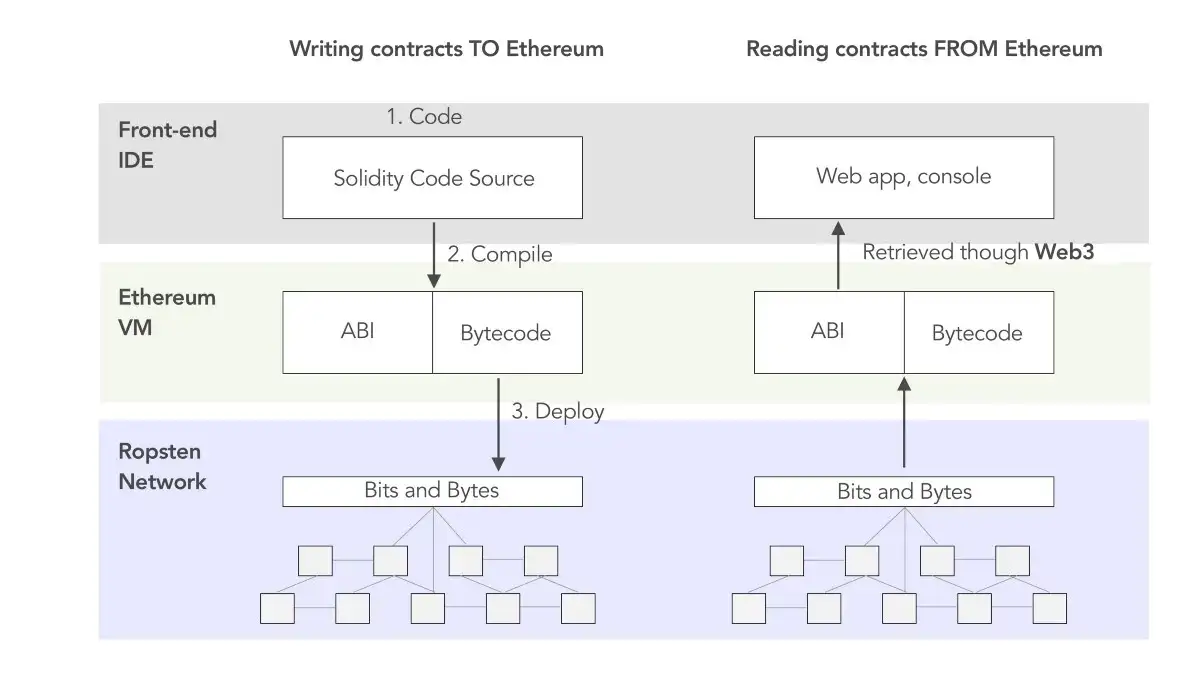
\includegraphics[width=1\textwidth]{img/Cap2/ethereum contracts.png}
    \caption{Implantação de um contrato inteligente em uma \emph{testnet} \cite{eiki_2019}}
    \label{fig:contrato_inteligente}
\end{figure}

Devido ao seu suporte de linguagens Turing-completas, a plataforma Ethereum abre margem para certos problemas computacionais \cite{Antonopoulos2018-jt}: por definição, um programa de computador Turing-completo é incapaz de prever seu fluxo de execução. Em outras palavras, é impossível um algoritmo saber quando sua execução irá terminar \cite{Sipser2012-gl}. Portanto, cenários em que execuções muito longas ocorrem, tal como a execução repetida de um mesmo trecho de código em um número exorbitante de vezes (os chamados loops infinitos), são imprevisíveis. Em um ambiente de execução distribuído, isto pode alavancar consequências indesejáveis, sobretudo desperdício de recursos computacionais e problemas de desempenho nos nós pertencentes a esse sistema. 
Para tratar deste problema, a plataforma Ethereum implementa um mecanismo chamado gas. Ao executar um contrato inteligente na EVM, cada comando do contrato invoca instruções do processador da máquina utilizada, como somar dois valores e persistir um dado. A partir daí, realiza-se um cálculo de gas com base no número de instruções utilizadas para efetuar a transação. Cada transação enviada deve conter obrigatoriamente um limite máximo de gas que está disposta a consumir para concretizar a operação. Se a quantidade de gas consumido exceder a quantidade de gas disponível, a execução do contrato é terminada. Desta forma, a rede garante limites para o uso de recursos computacionais, prevenindo abusos e gastos desnecessários. O gas é obtido com o uso da criptomoeda Ether \cite{EthereumGas}.

 Para realizar transações na rede, são utilizados valores fracionados da moeda Ether. Isso ocorre devido ao alto valor da criptomoeda: na primeira semana de fevereiro de 2023 a cotação de um único Ether era, em média, R\$ 8.400,00, o que equivale a aproximadamente US\$ 1.630,00. Devido ao valor diminuto de Ether necessário para realizar transações, foram criadas subdivisões para diferentes escalas da moeda, cada uma delas possuindo um nome padronizado pelo SI (Sistema Internacional de Unidades) junto de nomes coloquiais, fazendo homenagem a grandes pesquisadores da área de computação e da criptografia \cite{Antonopoulos2018-jt}. A menor unidade da criptomoeda é o \emph{wei}, sendo também o valor base utilizado na rede descentralizada.

 \begin{table}[H]
 \centering
\begin{tabular}{llll}
\hline
\multicolumn{1}{|l|}{Valor em wei} & \multicolumn{1}{l|}{Magnitude} & \multicolumn{1}{l|}{Nome coloquial} & \multicolumn{1}{l|}{Nome no SI} \\ \hline
\multicolumn{1}{|l|}{1} & \multicolumn{1}{l|}{1} & \multicolumn{1}{l|}{wei} & \multicolumn{1}{l|}{Wei} \\ \hline
\multicolumn{1}{|l|}{1,000} & \multicolumn{1}{l|}{10\textasciicircum{}3} & \multicolumn{1}{l|}{Babbage} & \multicolumn{1}{l|}{Kilowei/femtoether} \\ \hline
\multicolumn{1}{|l|}{1,000,000} & \multicolumn{1}{l|}{10\textasciicircum{}6} & \multicolumn{1}{l|}{Lovelace} & \multicolumn{1}{l|}{Megawei/picoether} \\ \hline
\multicolumn{1}{|l|}{1,000,000,000} & \multicolumn{1}{l|}{10\textasciicircum{}9} & \multicolumn{1}{l|}{Shannon} & \multicolumn{1}{l|}{Gigawei/nanoether} \\ \hline
\multicolumn{1}{|l|}{1,000,000,000,000} & \multicolumn{1}{l|}{10\textasciicircum{}12} & \multicolumn{1}{l|}{Szabo} & \multicolumn{1}{l|}{Microether} \\ \hline
\multicolumn{1}{|l|}{1,000,000,000,000,000} & \multicolumn{1}{l|}{10\textasciicircum{}15} & \multicolumn{1}{l|}{Finney} & \multicolumn{1}{l|}{Milliether} \\ \hline
\multicolumn{1}{|l|}{1,000,000,000,000,000,000} & \multicolumn{1}{l|}{10\textasciicircum{}18} & \multicolumn{1}{l|}{Ether} & \multicolumn{1}{l|}{Ether} \\ \hline
 &  &  &  \\
 &  &  &     
\end{tabular}
\caption{Valores monetários da criptomoeda Ether}
    \label{tab:tabela_valores_ether}
\end{table}


\subsection{\emph{Testnet}}
Abreviação de \emph{test network}, é uma rede utilizada para simular o comportamento da rede principal da plataforma Ethereum \cite{Antonopoulos2018-jt}. Como são redes paralelas, as \emph{testnets} são utilizadas para a realização de testes diversos, como transações, implantação e depuração de contratos antes destes serem migrados para a rede principal. As criptomoedas de uma \emph{testnet} não possuem valor real e podem ser facilmente adquiridas por via de \emph{faucets} (torneiras) de ether \cite{Dannen2017-eb}, servidores que transferem ether de teste à uma conta de uma \emph{testnet}.

\section{Segurança da Informação}
Os pilares da segurança de informação se baseiam na chamada tríade CIA (do inglês \emph{confidentiality}, \emph{integrity} e \emph{availability}). \cite{Nakamura2016} afirma que todas essas propriedades devem ser protegidas como um todo, e não isoladamente.

\begin{itemize}
    \item \textbf{Confidencialidade}: restringir dados e informações confidenciais a entidades não autorizadas. Também engloba a noção de privacidade, dando a estas entidades a autonomia de saber como, quais são e por quem seus dados estão sendo utilizados e de decidir se suas informações poderão ser acessadas, perante consentimento.
    \item \textbf{Integridade}: garantir que as informações transmitidas e armazenadas dentro do sistema não sofram nenhum tipo de adulteração, permitindo alterações somente a entidades previamente autorizadas.
    \item \textbf{Disponibilidade}: garantir que o sistema computacional consiga operar de forma normal e ininterrupta, sem haver nenhum tipo de inatividade que prejudique seus usuários.
\end{itemize}

Defronte destas definições, \cite{Stallings2015} vai além e lista adicionalmente os conceitos de autenticidade e responsabilização:
\begin{itemize}
    \item \textbf{Autenticidade}: a capacidade de uma entidade ser verificada e confiável, promovendo seguridade em meio a uma transação. Com ela conseguimos averiguar a identidade da entidade comunicante e saber se ela advém de uma fonte confiável ou não
    \item \textbf{Responsabilização}: a capacidade de figurar dentro de um sistema computacional os indivíduos responsáveis por suas ações, provendo assim irretratabilidade e meios de averiguar as transações realizadas. É necessária pois sistemas totalmente seguros ainda não são uma realidade.
\end{itemize}

\subsection{Criptografia}
A área de criptografia é constituída pelos muitos esquemas utilizados para encriptação de uma mensagem \cite{Stallings2015}. O processo de cifração consiste em transformar uma mensagem originalmente inteligível em uma mensagem cifrada por meio de uma série de substituições e transformações com o uso de um algoritmo. Blockchains usam as chamadas funções de \emph{hash} em seu funcionamento. Funções de \emph{hash} são funções que recebem uma determinada informação de entrada e produzem como saída uma cifra única dentro de sua capacidade (espaço de chaves). Em especial, usa-se a função SHA-256 da família de funções \emph{Secure Hash Algorithm} para produzir identificadores únicos na Blockchain, também chamados de endereços, que agem como uma assinatura digital de cada bloco da rede. Uma característica essencial das funções de \emph{hash} é a resistência a colisão, uma propriedade que garante que é computacionalmente inviável achar duas entradas distintas que resultem em um mesmo \emph{hash}. Esta propriedade constitui um dos pilares de segurança da Blockchain \cite{Karame2016-qb}.

\section{\emph{Logs}}
Um \emph{log} é uma mensagem gerada pelo sistema em resposta a algum tipo de estímulo \cite{Chuvakin2013-za}. Estes estímulos dependem do contexto e podem ser diversos, indo desde o simples login de um usuário em um ambiente Unix até mensagens de falha de hardware. O termo \emph{logs} costuma ser usado para expressar uma coleção de mensagens de \emph{log} referentes a um determinado uso. Podem ser armazenadas de diferentes maneiras, como arquivos de texto ou tabelas em um banco de dados relacional. Mensagens podem ser classificadas como:

\begin{itemize}
    \item \textbf{Informacionais}, projetadas para comunicar a usuários e administradores de algum acontecimento benigno;
    \item \textbf{Debug}, implantadas em sistemas de software com o intuito de auxiliar desenvolvedores de software a identifiar problemas com a aplicação;
    \item \textbf{Aviso}, usada em situação em que recursos podem estar faltando mas não são explicitamente necessários para o funcionamento do sistema;
    \item \textbf{Erro}, usada para notificar erros diversos que podem ocorrer em um sistema
    \item \textbf{Alerta}, utilizado para indicar o acontecimento de algo de interesse no sistema.
\end{itemize}

Cada mensagem de \emph{log} deve conter os seguintes elementos básicos: \emph{timestamp}, fonte e dados. Independente de como são armazenadas, as mensagens deverão conter estes itens. A \emph{timestamp} diz respeito a quando a mensagem foi gerada. A fonte, tipicamente um endereço IP ou \emph{hostname}, se refere ao sistema que gerou a mensagem de \emph{log}. Os dados são referentes à informação em si que o sistema deseja persistir, não possuindo padronização e nem representação fixa \cite{Chuvakin2013-za}.

\section{Auditoria}
Segundo \cite{Chuvakin2013-za}, auditoria é um processo que verifica se um sistema ou processo está funcionando como esperado. São chamados de auditores aqueles que realizam tarefas de auditoria, sendo responsáveis pelo bom funcionamento de controles internos \cite{Champlain2003-za} de empresas e organizações com o objetivo de mitigar riscos. Os auditores atuam aplicando julgamentos baseados em experiência e conhecimento para gerenciar os riscos possíveis em um contexto organizacional. O ideal é que todas as organizações passem por avalizações de risco e implementem maneiras de lidar com possíveis incidentes. A necessidade por auditoria sempre existiu, mas a sua urgência tem aumentado \cite{Champlain2003-za}, sobretudo por conta de ataques cibernéticos.

\emph{Logs} integram parte do processo de auditoria, implementando políticas de não repúdio (ou irretratabilidade) por meio das chamadas trilhas de auditoria. Uma trilha de auditoria é o registro de todas as ações realizadas por uma entidade em um sistema. Desta forma, toda e qualquer ação que seja executada em uma aplicação terá a garantia de que estará embasada e vinculada a um determinado usuário, atribuindo-lhe a responsabilidade pelo ato cometido. 

Define-se como trilha de auditoria um registro de todas as ações, eventos ou atividades realizadas por um usuário em um sistema \cite{privacytech_2020}. Englobam-se operações como criação de registros, bem como modificação e exclusão. Devido ao possível alto número de registros gerados numa base diária em um sistema, deve-se empregar técnicas para um rastreamento preciso e eficaz.

Segundo \cite{privacytech_2020}, a trilha de auditoria pode ser usada para diferentes finalidades:

\begin{itemize}
    \item Segurança da informação - a partir da trilha de auditoria é possível identificar que algo de errado aconteceu no sistema. Isto é possível por meio do armazenamento e rastreio de atividades de ações.

    \item Conformidade regulamentar - para dar a garantia de que o sistema é seguro e de que está em conformidade com normas e regulamentos diversos.

    \item Análise forense digital - a possibilidade de descobrir quem e porquê realizou determinada ação, com a capacidade de provar que a entidade responsável realmente realizou a ação.

    \item Integridade dos dados - a trilha de auditoria permite a reconstrução de dados que foram modificados e a hora em que foram modificados.

    \item Análise de negócios - os \emph{logs} fornecem uma visão geral acerca do funcionamento do negócio, já que a trilha de auditoria contém os dados que refletem diretamente aos processos do negócio.

    \item Detecção de fraudes e anomalias - devido à coleta de \emph{logs}, é possível a identificação de fraudes e anomalias ocorridas no sistema.
\end{itemize}


\section{Teste de \emph{software}}
Teste de \emph{software} é a prática de validar que o comportamento de uma aplicação seja aquilo que se espera \cite{Mohan2022-ch}. \cite{Pressman2021-jj}, por sua vez, define teste como um conjunto de atividades que podem ser planejadas com antecedência e executadas sistematicamente. A utilidade do teste de \emph{software} no processo de desenvolvimento é garantir qualidade ao código produzido. Não existe garantia de que todo \emph{software} seja totalmente livre de erros, então tem-se a necessidade de testar artefatos de \emph{software} para identificar possíveis erros inseridos durante sua construção.

Dois dos principais métodos de teste de \emph{software} são o teste de caixa-branca e o teste de caixa-preta. O teste de caixa-branca, também conhecido como teste estrutural, é uma abordagem de testes em que detalhes de implementação do código-fonte são conhecidos e estruturas internas do \emph{software} são testadas. Fluxos de controle costumam ser um dos focos desta abordagem. O teste de caixa-preta, também chamado de teste funcional, tem por foco os requisitos funcionais do \emph{software} \cite{Pressman2021-jj}. A partir de diferentes dados de entrada obtém-se diferentes tipos de saídas, que são validadas com base nos requisitos da aplicação. As técnicas de caixa-branca e caixa-preta não são mutuamente exclusivas, ambas têm diferentes focos de teste e se complementam.

Existem diversos tipos de testes que podem ser realizados em um sistema, possuindo diferentes escopos e aplicabilidades. Dois deles são foco deste trabalho: testes de unidade e testes de integração. Os testes de unidade se baseiam em testar as menores unidades de um sistema, que pode ser um método, uma função ou um componente, e garantir que ele funcione adequadamente. Já os testes de integração se referem a testes que são direcionados a sistemas que possuem diferentes módulos interagindo entre si. Mesmo que cada um dos módulos funcione de maneira correta individualmente, sua conjunção pode apresentar falhas. \cite{Pressman2021-jj} sugere que isto ocorre devido a falhas de interfaces, que podem ocasionar perda de dados, consequentemente acarretando em comportamentos inesperados em todo o conjunto de \emph{software}.